\documentclass[tikz,border=5pt]{standalone}
\usepackage[T1]{fontenc}
\usepackage{lmodern}
\usetikzlibrary{arrows.meta,positioning,fit}
\begin{document}
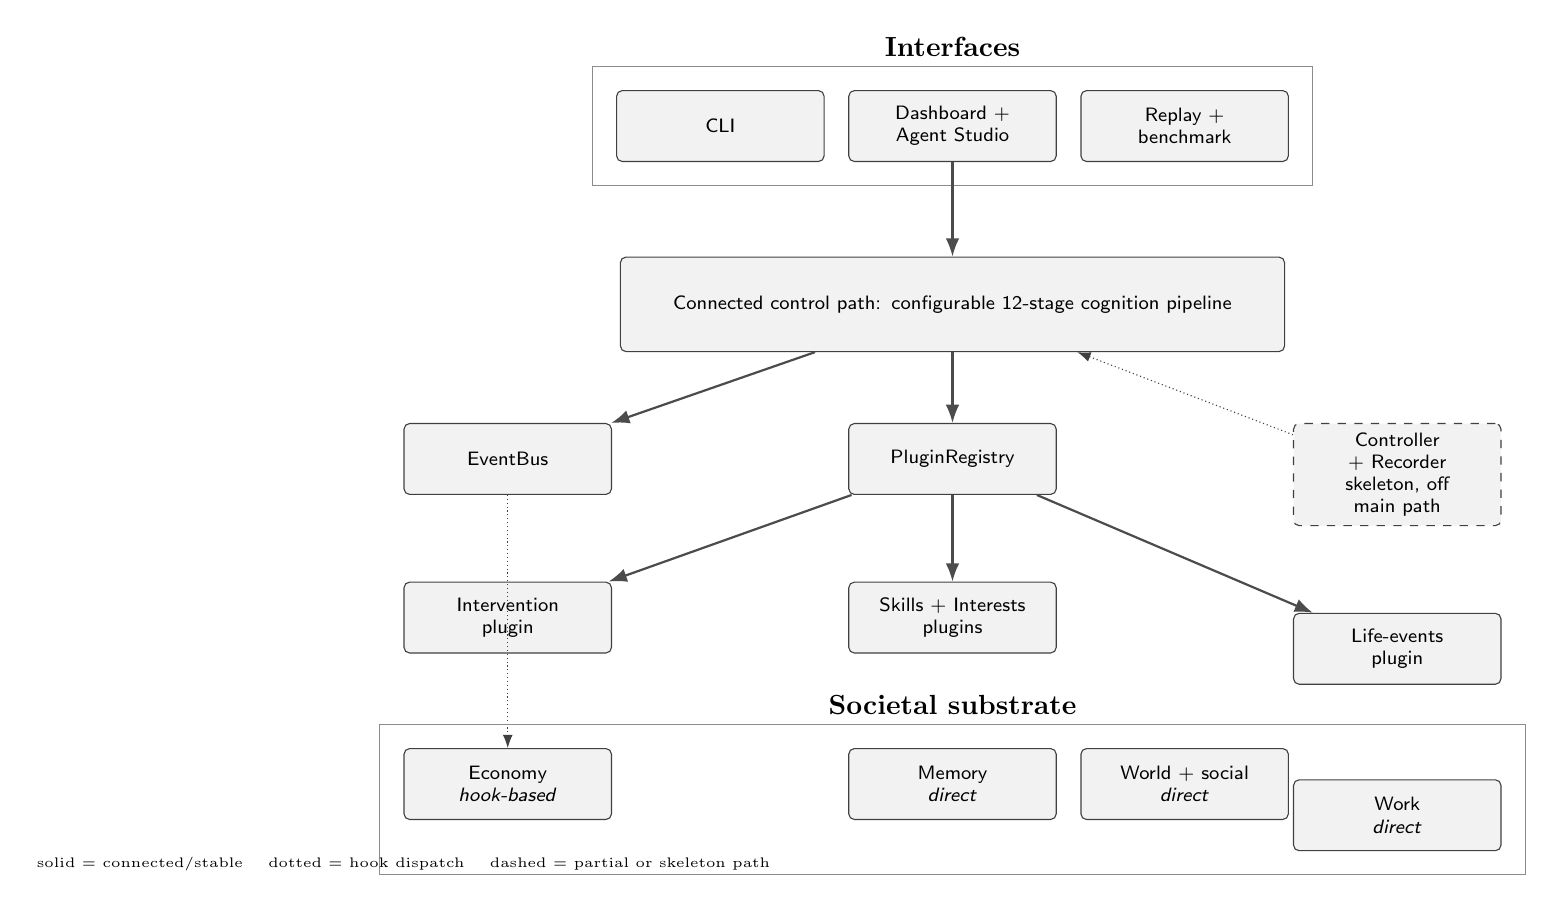
\begin{tikzpicture}[font=\sffamily\scriptsize,>=Latex,
 layer/.style={draw=black!75,rounded corners=2pt,fill=black!5,minimum height=9mm,align=center},
 item/.style={layer,text width=24mm}, flow/.style={->,thick,black!70},
 direct/.style={->,black!60}, hook/.style={->,densely dotted,black!75}]
\node[item] (cli) {CLI};
\node[item,right=3mm of cli] (dash) {Dashboard +\\Agent Studio};
\node[item,right=3mm of dash] (replay) {Replay +\\benchmark};
\node[draw=black!45,fit=(cli)(replay),inner sep=3mm,label={[font=\bfseries]above:Interfaces}] {};

\node[layer,below=12mm of dash,text width=82mm,minimum height=12mm] (pipe)
 {Connected control path: configurable 12-stage cognition pipeline};
\node[item,below left=9mm and 1mm of pipe] (bus) {EventBus};
\node[item,below=9mm of pipe] (registry) {PluginRegistry};
\node[item,below right=9mm and 1mm of pipe,dashed] (skeleton) {Controller + Recorder\\skeleton, off main path};
\draw[flow] (dash) -- (pipe);
\draw[flow] (pipe) -- (bus);
\draw[flow] (pipe) -- (registry);
\draw[hook] (skeleton) -- (pipe);

\node[item,below=11mm of bus] (policy) {Intervention\\plugin};
\node[item,below=11mm of registry] (skills) {Skills + Interests\\plugins};
\node[item,below=11mm of skeleton] (life) {Life-events\\plugin};
\draw[flow] (registry) -- (policy);
\draw[flow] (registry) -- (skills);
\draw[flow] (registry) -- (life);

\node[item,below=12mm of policy] (economy) {Economy\\\textit{hook-based}};
\node[item,below=12mm of skills] (memory) {Memory\\\textit{direct}};
\node[item,right=3mm of memory] (world) {World + social\\\textit{direct}};
\node[item,below=12mm of life] (work) {Work\\\textit{direct}};
\draw[hook] (bus) -- (economy);
\node[draw=black!45,fit=(economy)(work),inner sep=3mm] (substrate) {};
\node[font=\bfseries,anchor=south] at (substrate.north) {Societal substrate};

\node[font=\tiny,anchor=west,below=8mm of economy.west] {solid = connected/stable \quad dotted = hook dispatch \quad dashed = partial or skeleton path};
\end{tikzpicture}
\end{document}
